\documentclass{article}
\usepackage{geometry}
\usepackage{setspace}
\usepackage{array}
\usepackage{graphicx}
%\graphicspath{{/home/utkarsh/}}
\geometry{left=0.5in,right=0.5in,top=0.6in,bottom=0.5in}
\usepackage{graphicx}
\begin{document}
\pagenumbering{gobble}
\sffamily
\begin{flushleft}
{\Huge{Utkarsh Agarwal}}
\end{flushleft}
\vspace{-1cm}
\begin{figure}[ht]
\begin{minipage}[b]{0.35\linewidth}
\begin{flushleft}
{\small Second Year Undergraduate \newline
       Dept. of Computer Science and Engineering\\
       IIT Kanpur\newline
       Ph:7388447711\\
       E-mail: utkarsha@iitk.ac.in\newline }
\end{flushleft}
\end{minipage}
\hspace{4cm}
\begin{minipage}[b]{0.55\linewidth}
\centering
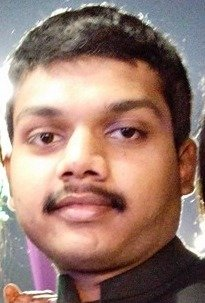
\includegraphics[width=3.5cm,height=3.5cm]{image.jpg}
\end{minipage}
\end{figure}
{\Large Educational Qualifications}
\newline
\newline
\begin{tabular}{| l | l | l |l|}
\hline
Year         & Degree & Institution & CPI/Percentage\\ \hline
2013-2017(Expected) & B.Tech, Computer Science and Engineering & Indian Institute of Technology, Kanpur & 9.6/10*\\ \hline
2013 & AISSCE(CBSE 12th) & DAV Public School, Kota & 92.4 \\ \hline
2011 & AISSE(CBSE 10th) & Mayoor School,Ajmer & 10/10\\ \hline
\end{tabular}
*At the beginning of the fourth semester \newline\newline\newline
{\Large Scholastic Achievements}
	\begin{itemize}
\item Secured All India Rank (AIR) \textbf {132} (top 0.09\%) in \textbf {IIT Joint Entrance Examination (JEE) 2013} 
\item Selected to appear in \textbf{INJSO, 2009 and INChO, 2012}: National Olympiads conducted by HBCSE, India for being amongst the \textbf{top 300 in India}.
\item Amongst the \textbf{top 100} out of 1000 selected from all over India for \textbf{NTSE Scholarship, 2009}: a prestigious scholarship funded by NCERT, Delhi.
\item Awarded a certificate for being the amongst the \textbf{top 1 percentile in India} in  NSEP.
\item Awarded Merit Certificate by CBSE for securing \textbf{10/10 CGPA} in 10th class.
	\end{itemize}
\vspace{10pt}
{\Large Projects}
\begin{itemize}
\item {\large Scotland Yard Computer Game}\newline
(Under Programming Club, IITK)\hfill (May-June, 2014)
	\begin{itemize}
	\item Designed GUI of the game using Pygame library in Python
	\item Used Graph Theory to link the map of the city with a graph for use in AI
	\item Wrote the AI of the game using Minimax Algorithm in Python

	\item Used sockets library to extend it to a Multiplayer Version that can be played on LAN
	\end{itemize}
	
\item {\large News Article Classifier}\newline
(Under ACA, IITK)\hfill (Jan-Feb 2014)
	\begin{itemize}
	\item Used Beautiful Soup library in Python to extract news articles from websites
	\item Used the Reuters Corpus for classification of words into different categories
	\item Used the NLTK library to write a classifier that classified news articles on the basis of topics it was written upon i.e. Politics, Sports, Science, etc.
	\end{itemize}
	
\item {\large CAM Hammer}\newline	
(As part of TA201: Manufacturing Processes)\hfill (Aug-Nov 2014)
	\begin{itemize}
	\item Awarded 2nd best Sectional Project
	\item Building a miniature CAM Hammer using Cast Iron
	\item Processes of welding, brazing, casting and sheet metal forming are being primarily used
	\end{itemize}
	\end{itemize}
\vspace{100pt}	
{\Large Relevant Courses}
\newline
\newline
\begin{tabular}{l l l l}
Course & Course Name & Credits & Grade\\
\multicolumn{4}{c}{\textbf{2013-2014/I(first)}}\\
ESC101& Fundamentals of Computing & 14\hspace{100pt} & B\hspace{10pt} \\ 
MTH101& Real Analysis & 11 & B \\
PSY152& Introduction to Psychology & 11 & B\\
\multicolumn{4}{c}{\textbf{2013-2014/II(second)}}\\ 
MTH102\hspace{30pt} & Linear Algebra & 11 & B\\
PHY102&  Introduction to Mechanics & 11 & B\\
TA101 &  Compulsory Engineering Graphics\hspace{90pt} & 9 & B\\
\multicolumn{4}{c}{\textbf{2014-2015/I(first)}}\\ 
CS210 & Data Structure and Algorithms & 12 & B \\ 
CS201 & Discrete Mathematics & 9 & B\\ 
ESC201 & Introduction to Electronics & 14 & B
\end{tabular}
\newline
\newline
\newline
{\Large Technical Skills}
\begin{itemize}
\item Programming Languages: C, C++,Python
\item OS: Windows, Linux
\item Other: Git, Latex
\end{itemize} 
\vspace{10pt}
{\Large Extra-Curricular Achievements}
\begin{itemize}
\item Programming
	\begin{itemize}
	\item Active member of Programming Club, IITK
	\item Enthusiastic Competitive Programmer
	\end{itemize}
\item English Literary Activities / Debating / Oration
	\begin{itemize}
	\item Adjudged Best Debater in Middle and Senior Section in School
	\item Represented School in various Inter School Debate Competitions
	\item Stood 1st in Galaxy, an Intra IITK cultural fest 
	\end{itemize}
\item Quiz
	\begin{itemize}
	\item School Quiz Team Captain
	\item Represented School in various Inter School Quiz Competitions
	\end{itemize}
\item Tennis
	\begin{itemize}
	\item U-17 School Tennis Team Captain
	\end{itemize}
\item Member of Alumni Contact Program(ACP), IITK : A program aimed at improving Alumni Relations
\end{itemize}
\vspace{10pt}
{\Large Positions of Responsibility}
\begin{itemize}
\item Senior Executive, Public Relations, Antaragni’14
	\begin{itemize}
	\item Invited eminent personalities for Antaragni
	\item Helped in managing events and looked after the guests
	\end{itemize}
\item Academic Mentor
\begin{itemize}
\item Academic Mentor of ESC101 to 1st year students
\end{itemize}
\end{itemize}
\end{document}
